\subsection{Werkzeuge}
Die Entwicklung von Anwendungen für Mikrocontroller bietet eine Reihe von Besonderheiten, insbesondere durch die begrenzte Beobachtbarkeit und Kontrolle zur Laufzeit der Ausführung. Entsprechend müssen auch die genutzten Werkzeuge über spezielle Funktionalitäten verfügen, um die Entwicklung trotzdem effizient zu gestalten. Die in dieser Projektgruppe eingesetzten Tools sollen nun im Folgenden kurz vorgestellt werden.

\subsubsection{Atmel Studio}
Atmel Studio (vormals AVR Studio) ist eine integrierte Entwicklungsumgebung für eingebettete Systeme, insbesondere für die Atmel-eigenen Mikrocontrollerfamilien.
Es basiert auf Microsoft Visual Studio, eignet sich aber insbesondere für die Entwicklung von Software für eingebettete 8- und 32-Bit Controller mit C, C++ und Assembler.
Kern der Anwendung ist ein Cross-Compiler, der es erlaubt, ausführbare Binärdateien direkt für die Zielhardware zu kompilieren.

\autoref{fig:avrstudio1} zeigt einen Screenshot vom Atmel Studio. Das Hauptfenster links zeigt die Code-Ansicht mit farblich markierter Code-Struktur, während rechts die Dateistruktur des Projekts abgebildet ist.

\begin{figure}[!t]
  \centering
    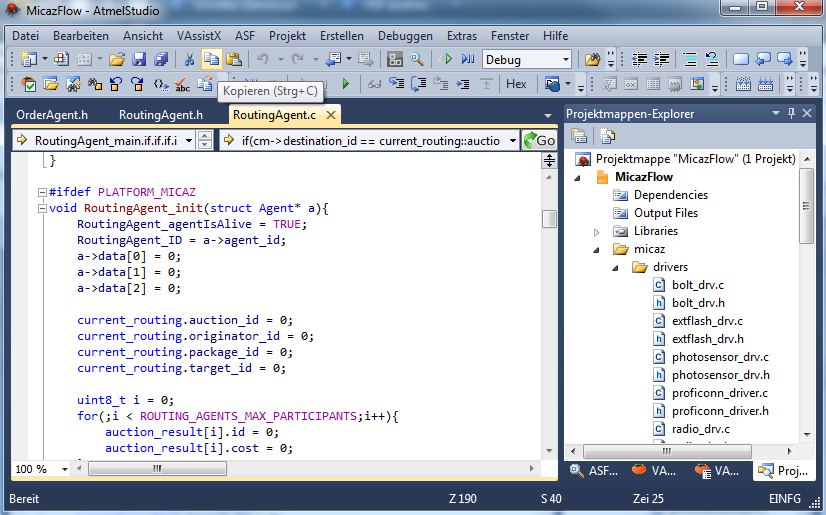
\includegraphics[width = 0.85\textwidth]{flow/AVRStudio_1.png}
    \caption{Entwicklungs-Ansicht des Atmel Studio}
    \label{fig:avrstudio1}
\end{figure}

\begin{figure}[!h]
  \centering
    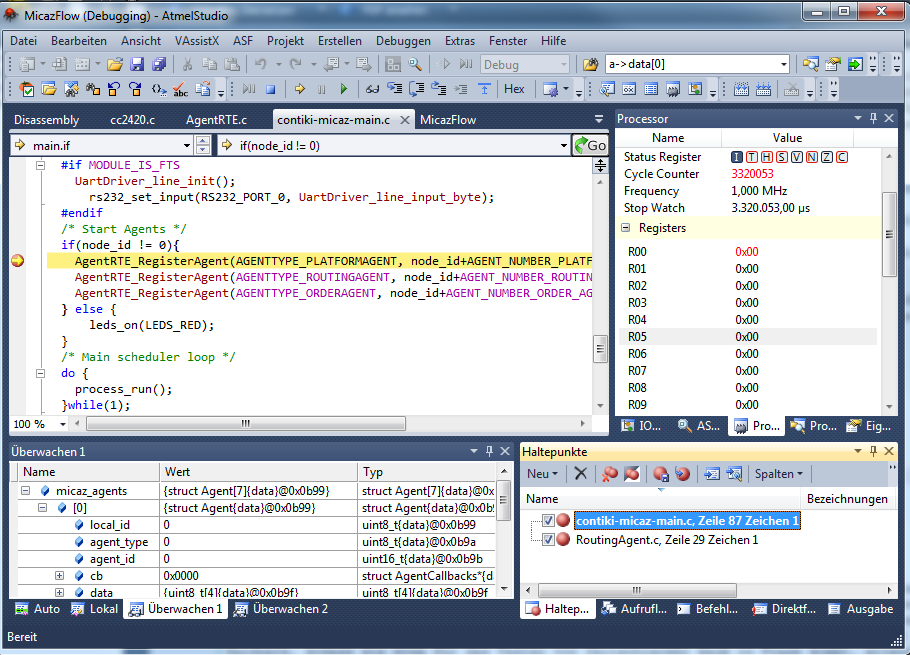
\includegraphics[width = 0.85\textwidth]{flow/AVRStudio_2.png}
    \caption{Debugging-Ansicht des Atmel Studio}
    \label{fig:avrstudio2}
\end{figure}

Neben dem Cross-Compiler beinhaltet das Atmel Studio auch einen Simulator, der es erlaubt, die Ausführung der entwickelten Software auf der Zielhardware zu simulieren. Dabei können Register, Hauptspeicher und Pins des Zielcontrollers beobachtet und Haltepunkte im Code gesetzt werden. Die Simulation ist um ein vielfaches langsamer als die Ausführung auf echter Hardware, sodass sie etwa für das Testen von Zeitschranken kaum in Frage kommt, allerdings gibt sie einen ersten Eindruck von der Funktionalität der eigenen Anwendung.

\autoref{fig:avrstudio2} zeigt einen Screenshot der Debugging-Ansicht des Atmel Studios. Links oben ist das Code-Fenster zu sehen. Die Ausführung ist gerade angehalte, sodass die nächste auszuführende Anweisung gelb markiert ist. Der rote Punkt links stellt einen Haltpunkt dar: Vor Abarbeitung der Anweisungen in dieser Zeile wird die Ausführung pausiert. Rechts oben befindet sich der \textit{Processor View}, der über Registerinhalte, Taktzyklen, Taktrate und weitere prozessorspezifische Details informiert. Unten links befindet sich das Überwachungsfenster, in dem die Werte von ein oder mehreren Variablen oder ganzen Strukturen beobachtet und verändert werden können. Rechts daneben sind schließlich alle Haltepunkte aufgeführt, die zur Zeit im Code definiert sind. Man unterscheidet dabei zwischen Programm- und Datenhaltepunkten. Programmhaltepunkte lösen immer dann aus, wenn bei der Ausführung die entsprechende Zeile im Code erreicht wird. Datenhaltepunkte hingegen lösen immer dann aus, wenn sich der Wert der angegebenen Speicherstelle beziehungsweise Variablen ändert.

\subsubsection{Atmel JTAGICE3}
\label{sec:JTAGICE3}
Die Probleme der simulationsbasierten Ausführung der entwickelten Anwendung sind vor allem die üblicherweise deutlich niedrigere Geschwindigkeit im Vergleich mit der Ausführung auf der Zielhardware und zum Anderen die fehlende Peripherie, sodass angeschlossene Sensoren, Aktoren oder andere Hardwarebausteine, wie der CC2420-Funkchip der \textsc{Mica}z-Module, nicht getestet werden können.

Eine Lösung bietet der Atmel JTAGICE3 \cite{AtmelJTAGICE3:2014:Online}, der über eine JTAG-Schnittstelle direkt auf die Zielhardware zugreifen und ihren Zustand auslesen und verändern kann. \textbf{JTAG} steht für \textit{Joint Test Action Group} und ist eine standardisierte (IEEE Standard 1149.1, siehe \cite{IEEE1149:2014:Online}) Schnittstelle für das Programmieren und das Debuggging von integrierten Schaltungen. Es erlaubt - ähnlich wie das simulationsbasierte Debugging - den direkten Zugriff auf Register- und Speicherwerte, allerdings erfolgt der Zugriff direkt auf der Hardware. Das bedeutet insbesondere, dass auch eingehende Drahtlos- beziehungsweise UART-Nachrichten, die über die externen Ports des Mikrocontrollers eingehen, direkt überwacht und ausgewertet werden können.

Dafür verfügt das \textsc{Mib}520 über eine Steckerleiste, den sogenannten Test Access Port (TAP). Dieser besteht aus fünf Steuerleitungen, die die Testausführung auf dem Mikrocontroller regeln:
\begin{itemize}
\item Test Clock (TCK)
\item Test Reset (TRST)
\item Test Mode Select (TMS)
\item Test Data In (TDI)
\item Test Data Out (TDO)
\end{itemize}

Darüber ist es möglich, bei leicht verminderter Taktfrequenz alle relevanten Informationen zur Laufzeit aus dem Mikrocontroller zu gewinnen oder gar Veränderungen an Register- und Speicherwerten vorzunehmen, sowie Haltepunkte zu setzen. Außerdem kann ein Mikrocontroller über den JTAGICE3 auch programmiert und sein Festspeicher (meist EEPROM oder Flash) beschrieben werden.

\begin{figure}[!h]
  \centering
    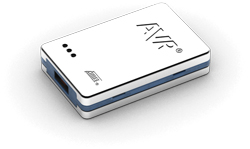
\includegraphics[width = 0.7\textwidth]{flow/jtagice3.jpg}
    \caption{Atmel JTAGICE3 \cite{AtmelJTAGICE3:2014:Online}}
    \label{fig:jtagice3}
\end{figure}

\autoref{fig:jtagice3} zeigt einen solches Gerät mit drei Kontrolllämpchen für Stromversorgung und Status, sowie dem zehn-poligen TAP-Konnektor (einige Pins werden für JTAG nicht genutzt, siehe oben).